\newpage

\section{Configurazione ambiente di lavoro}
In questa sezione verranno descritti gli strumenti utilizzati e consigliati per lo sviluppo dell'applicazione. Inoltre verranno descritte delle procedure per l'installazione e la configurazione degli stessi.
%
	\subsection{Requisiti di sistema}
	Essendo \progetto{} un'applicazione web, è necessaria una connessione ad internet per poterla utilizzare.
	\subsubsection{Dispositivi e browser supportati}
		Al momento della stesura di questo documento l'applicazione è supportata dai seguenti dispositivi:
		\begin{itemize}
			\item Window v10
			\item Linux Ubuntu10.04 e Debian 8.0
			\item MacOS v10.2
			\item Tablet - Asus P01MA con sistema operativo Android 6.0.1
			\item Tablet - iPad Air 2 con sistema operativo iOS 10.2
		\end{itemize}
		e dai seguenti browser:
		\begin{itemize}
			\item Chome v55
			\item Safari v10
			\item Firefox v5.3 per iOS 10.2
			\item Firefox v50
		\end{itemize}
	%
	\subsection{IDE: WebStorm}
	WebStormG è un IDE fornito dall'azienda JetBrains per lo sviluppo di applicazioni e siti web. Questo software permette di supportare lo sviluppatore nella realizzazione di prodotti web. Tra le principali funzionalità sono presenti:
	\begin{itemize}
		\item assistenza nella codifica dei principali framework web;
		\item auto-completamento per la sintassi di molti linguaggi (es. \js, HTML, CSS);
		\item gestione di progetti complessi;
		\item integrazione con i più popolari tool per lo sviluppo web;
		\item integrazione di un sistema di debugging per il codice \js;
		\item compatibilità con sistemi di build automatico.
	\end{itemize}
	Questo strumento è stato utilizzato durante l'attività di codifica e le principali motivazioni che hanno portato il gruppo alla sua scelta sono:
	\begin{itemize}
		\item strumento completo e professionale;
		\item licenza gratuita per studenti;
		\item integrabilità con strumenti per analisi statica e test;
		\item integrabilità con GitHub;
		\item cross-platform.
	\end{itemize}
	%
	\begin{table}[H]
		\centering
		\begin{tabular}{p{2cm}p{0.5cm}p{11.5cm}}
			\arrayrulecolor{lightgray}
			\toprule
			\textbf{Indirizzo download} & &
			\url{https://www.jetbrains.com/webstorm/download/}
			\\ \midrule
			\textbf{Versione installata} & &
			2017.1 o superiore
			\\ \bottomrule
		\end{tabular}
	\end{table}
	%
	\subsection{Gestore dei pacchetti}
		\subsubsection{Node.js} \label{nodejs}
		Node.js è una piattaforma event-driven per il motore \js{} V8, disponibile sulle principali piattaforme, anche se maggiormente performante su sistemi operativi UNIX-like.
		\begin{table}[H]
			\centering
			\begin{tabular}{p{2cm}p{0.5cm}p{11.5cm}}
				\arrayrulecolor{lightgray}
				\toprule
				\textbf{Indirizzo download} & &
				\url{https://nodejs.org/en/download/}
				\\ \midrule
				\textbf{Versione installata} & &
				6.9.5 o superiore
				\\ \bottomrule
			\end{tabular}
		\end{table}
		Consigliamo la versione stabile (LTS) di Node.js e non quella con le ultime features. Inoltre per verificare la versione attualmente installata, eseguire il seguente comando a terminale:
		\begin{center}
			\hicode{node -v}
		\end{center}
		%
		\subsubsection{npm} \label{npm}
		npm (node package manager) è il gestore di pacchetti di default utilizzato da Node.js. Questo strumento consente  l'installazione e la gestione di moduli esterni che forniscono funzionalità aggiuntive al sistema node di base, risolvendo varie dipendenze.
		Le principali motivazioni che hanno portato il gruppo alla scelta di questo strumento sono:
		\begin{itemize}
			\item larga diffusione;
			\item più di 400.000 pacchetti installabili;
			\item ampia documentazione.
		\end{itemize}
		\begin{table}[H]
			\centering
			\begin{tabular}{p{2cm}p{0.5cm}p{11.5cm}}
				\arrayrulecolor{lightgray}
				\toprule
				\textbf{Indirizzo download} & &
				\url{https://www.npmjs.com}
				\\ \midrule
				\textbf{Versione installata} & &
				4.2.0 o superiore
				\\ \bottomrule
			\end{tabular}
		\end{table}
		Per lo sviluppo di questo progetto è stato creato e configurato un apposito file che richiama l'installazione di tutti i pacchetti necessari. Di seguito viene descritta la procedura per l'installazione di quest'ultimo:
		\begin{enumerate}
			\item aver installato Node.js, oppure installarlo seguendo le istruzioni descritte in \ref{nodejs};
			\item aprire un terminale e posizionarsi all'interno della cartella del progetto, in modo da scaricare i pacchetti localmente . Se non presente, scaricarla tramite la procedura descritta nella sezione \ref{downloadProgetto};
			\item scrivere il comando 
			\begin{center}
				\hicode{npm install} \label{npminstall}
			\end{center}
			\item attendere il termine dell'installazione, che può durare anche qualche minuto in funzione della banda o della potenza del processore;
		\end{enumerate}
		Per vedere la lista dei pacchetti installati e controllarne la versione scrivere nel terminale all'interno della cartella del progetto \progetto:
		\begin{center}
			\hicode{npm list}
		\end{center}
	%
	\subsection{Browser}
		\subsubsection{Google Chrome}
		L'indirizzo per il download è valido per i seguenti sistemi operativi: Windows 10/8.1/8/7 64/32-bit, Mac OS X 10.9+, Linux
		\begin{table}[H]
			\centering
			\begin{tabular}{p{2cm}p{0.5cm}p{11.5cm}}
				\arrayrulecolor{lightgray}
				\toprule
				\textbf{Indirizzo download} & &
				\url{https://www.google.it/chrome/browser/desktop/index.html}
				\\ \midrule
				\textbf{Versione installata} & &
				55 o superiore
				\\ \bottomrule
			\end{tabular}
		\end{table}
		\subsubsection{Mozilla Firefox}
				L'indirizzo per il download è valido per i seguenti sistemi operativi: Windows 10/8.1/8/7 64/32-bit, Mac OS X 10.9+, Linux
		\begin{table}[H]
			\centering
			\begin{tabular}{p{2cm}p{0.5cm}p{11.5cm}}
				\arrayrulecolor{lightgray}
				\toprule
				\textbf{Indirizzo download} & &
				\url{https://www.mozilla.org/it/firefox/new/?scene=2}
				\\ \midrule
				\textbf{Versione installata} & &
				50 o superiore
				\\ \bottomrule
			\end{tabular}
		\end{table}
		\subsubsection{Safari}
		\begin{table}[H]
			\centering
			\begin{tabular}{p{2cm}p{0.5cm}p{11.5cm}}
				\arrayrulecolor{lightgray}
				\toprule
				\textbf{Indirizzo download} & &
				\url{Integrato nei Mac}
				\\ \midrule
				\textbf{Versione installata} & &
				10 o superiore
				\\ \bottomrule
			\end{tabular}
		\end{table}
	%
	\subsection{Download del progetto} \label{downloadProgetto}
	Il progetto è attualmente ospitato presso una repository privata su GitHub e quindi necessita l'autorizzazione da parte del grippo \zephyrus. Una volta ottenuta, si può procedere con la procedura seguente:
	\begin{enumerate}
		\item scaricare il progetto tramite il seguente link:
			\begin{center}
				\url{https://github.com/JordanGottardo/DeGeOP}
			\end{center}
			\begin{figure}[H]
				\centering 
				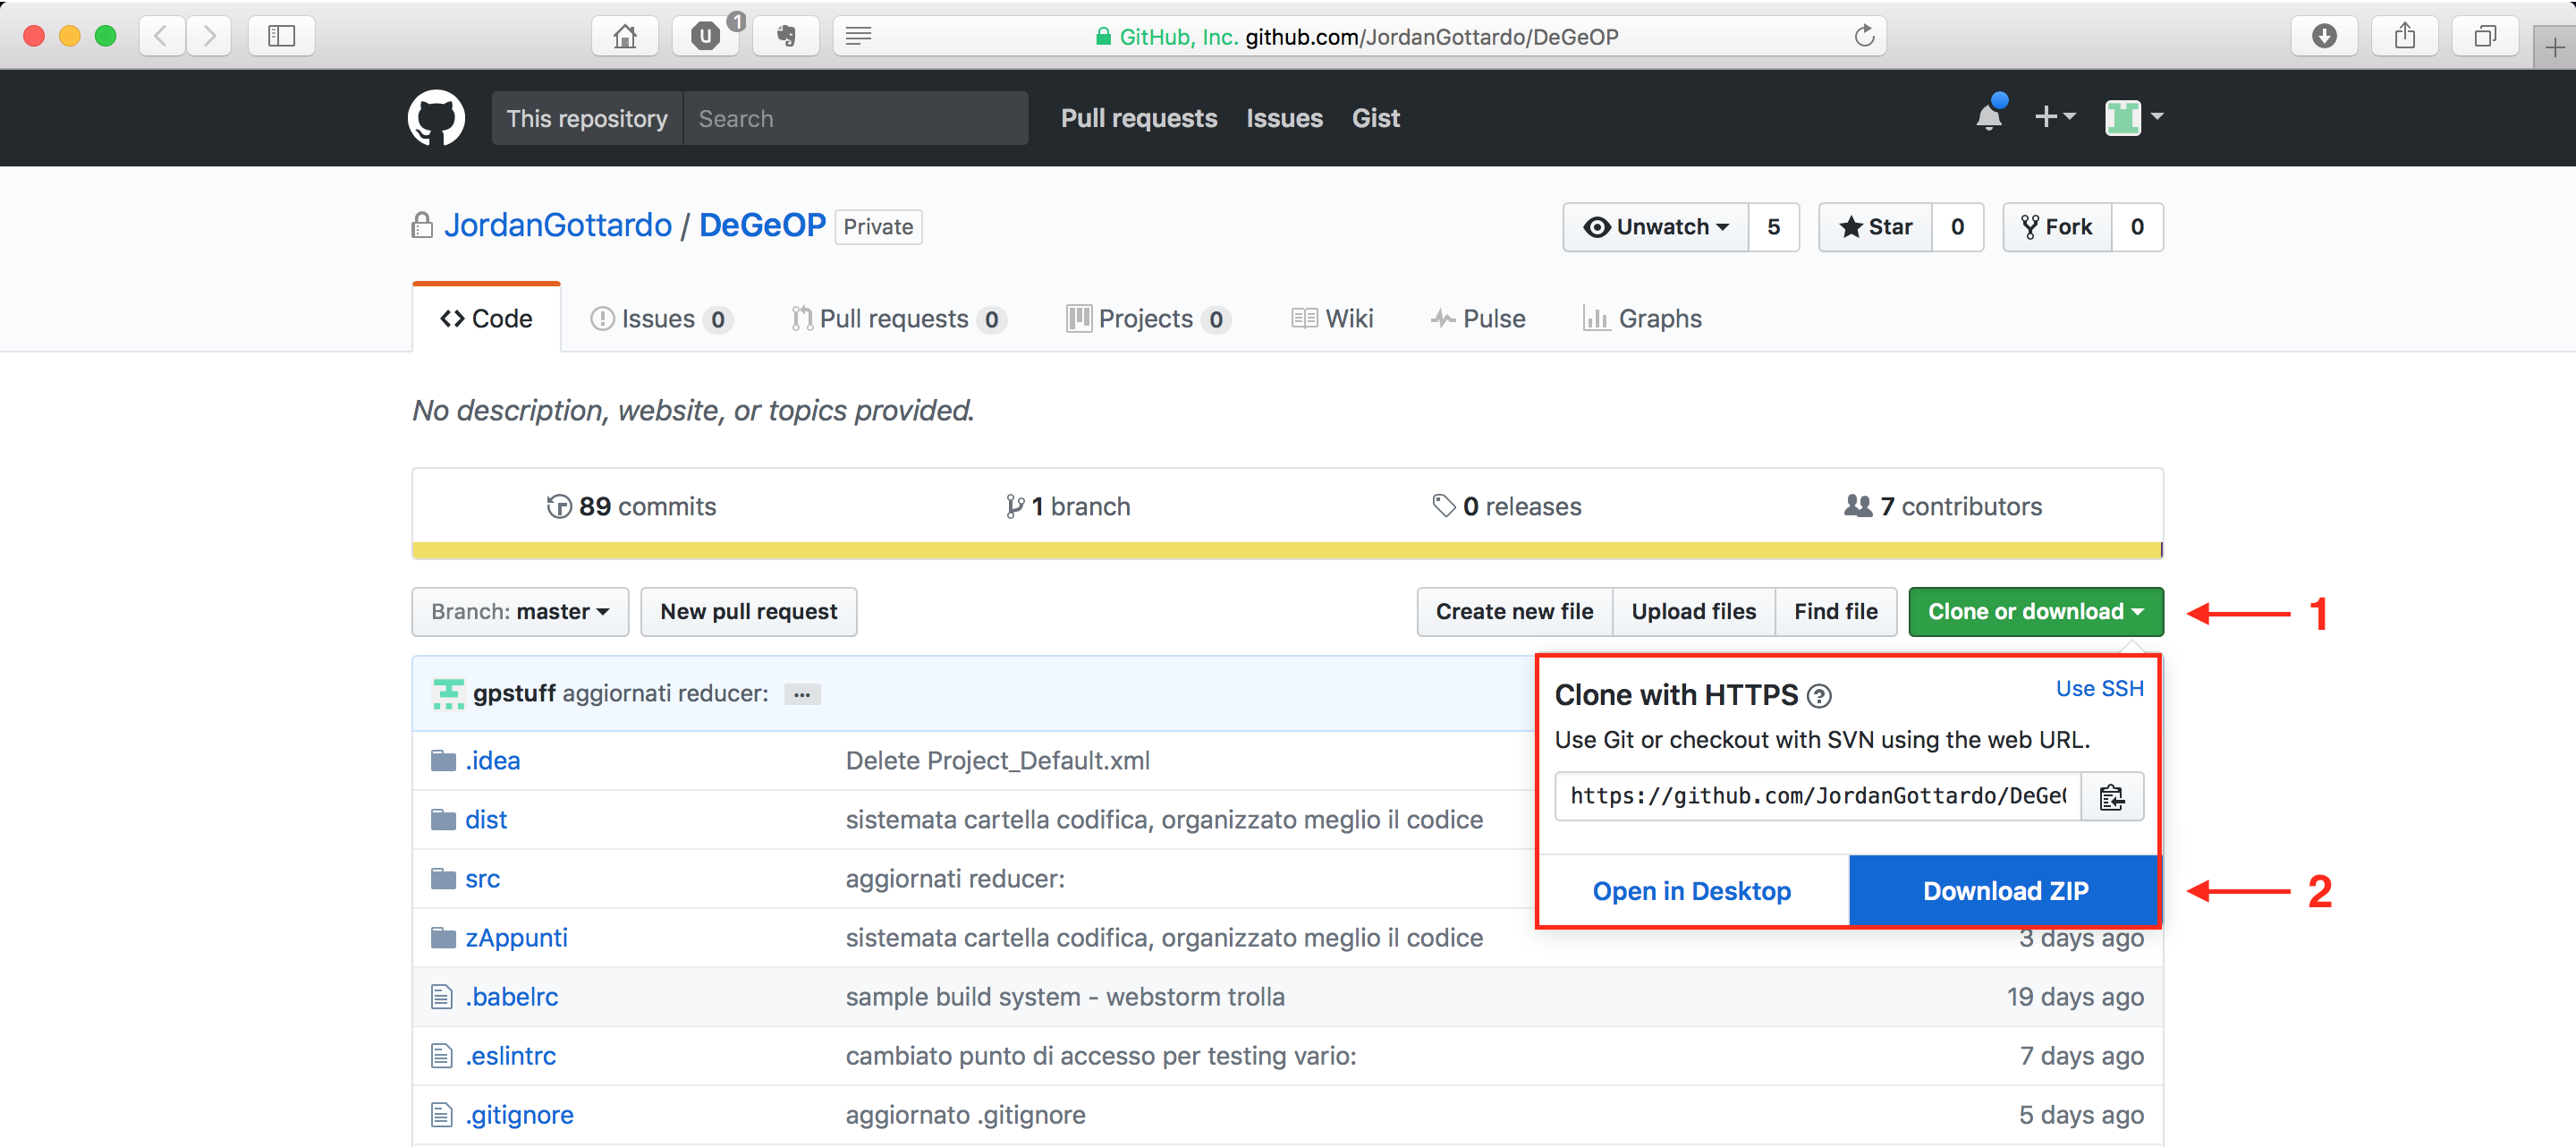
\includegraphics[width=1\columnwidth]{img/downloadProgetto.png}
				\caption{Download progetto \progetto dalla repository su GitHub}
			\end{figure}
		\item decomprimere il file \texttt{.zip} scaricato;
		\item avviare WebStorm e aprire il progetto, seguendo il menu: \hicode{File -> Open} e selezionare la cartella estratta al punto 2;
		\item (opzionale) dopo aver installato tutti i pacchetti con procedura \ref{npminstall}, è possibile configurare ESLint. Di seguito vengono descritti i passi per la configurazione su WebStorm:
			\begin{enumerate}
				\item aprire WebStorm;
				\item aprire il menu \hicode{File -> Preferences};
				\item entrare nel menu \hicode{Language \& Frameworks->JavaScript->Code Quality->ESLint};
				\item abilitare il tool essicurandosi di aver installato prima Node.js (vedi sezione \ref{nodejs});
				\item selezionare nel campo ESLint package il file che si trova all'interno del progetto \texttt{DeGeOp/node_modules/eslint};
			\end{enumerate}
			\begin{figure}[H]
				\centering 
				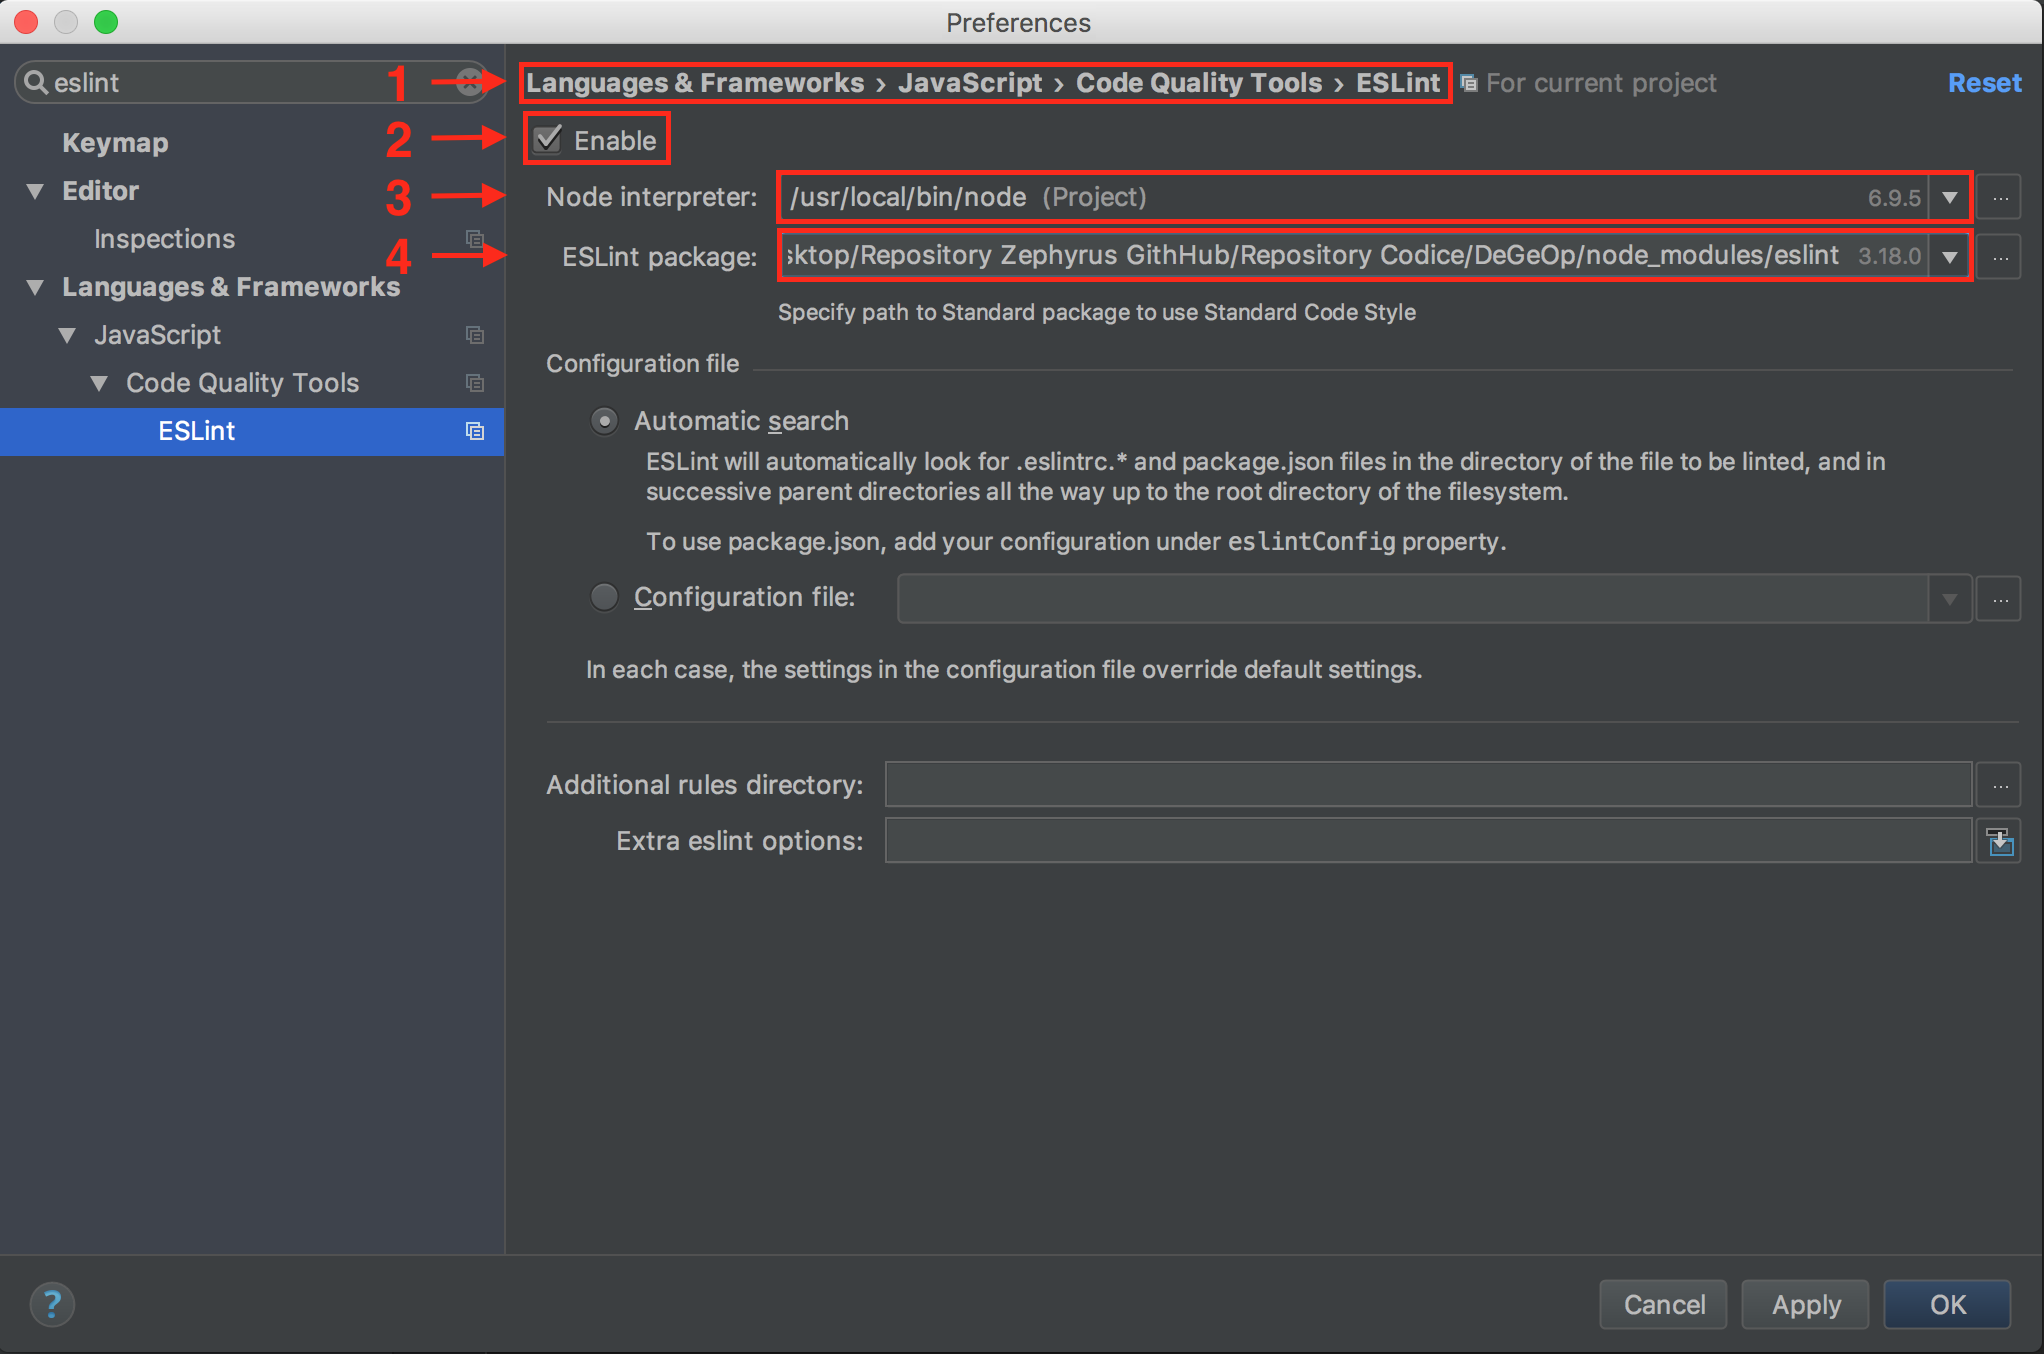
\includegraphics[width=1\columnwidth]{img/configESLint.png}
				\caption{Configurazione ESLint \progetto su WebStorm}
			\end{figure}
	\end{enumerate}
	
	%
	\subsection{Configurazione della VirtualBox}
	In accordo con il proponente abbiamo installato una macchina virtuale per effettuare il deploy e testare la nostra applicazione con il server di \riskapp{}. La procedura per configurare la macchina virtuale è la seguente:
	\begin{enumerate}
		\item scaricare e installare sul proprio computer Oracle VirtualBox dal sito ufficiale:
		\begin{center}
			\url{https://www.virtualbox.org/wiki/Downloads}
		\end{center} 
		\item scaricare il file immagine della macchina virtuale creata da \riskapp{},  dal seguente link, inserendo le apposite credenziali fornite dal proponente:
		\begin{center}
			\url{https://www.satellite1.info/u/Zephyrus.ova};
		\end{center} 
		\item aprire l'applicazione VirtualBox sul proprio computer;
		\item aprire il menù \hicode{File} e selezionare \hicode{Import Appliance};
		\item selezionare il file \hicode{Zephyrus.ova} scaricato nel punto 2 e cliccare su \hicode{Next};
		\item cliccare su \hicode{Import} e attendere la fine del processo;
		\item terminata l'importazione fare click destro sulla nuova macchina virtuale presente nell'elenco a sinistra e selezionare \hicode{Settings};
		\item selezionare la sezione \hicode{Network};
		\item nella tab \hicode{Adapter 1} modificare l'opzione \hicode{Attached to:} in \hicode{NAT} e cliccare \hicode{OK};
		\item la macchina virtuale è ora pronta all'uso.
	\end{enumerate}
	%